\documentclass[12pt]{beamer}
\usepackage{../Estilos/BeamerMAF}
\usepackage{../Estilos/ColoresLatex}
%Sección para el tema de beamer, con el theme, usercolortheme y sección de footers
\usetheme{CambridgeUS}
\usecolortheme{beaver}
%\useoutertheme{default}
\setbeamercovered{invisible}
% or whatever (possibly just delete it)
\setbeamertemplate{section in toc}[sections numbered]
\setbeamertemplate{subsection in toc}[subsections numbered]
\setbeamertemplate{subsection in toc}{\leavevmode\leftskip=3.2em\rlap{\hskip-2em\inserttocsectionnumber.\inserttocsubsectionnumber}\inserttocsubsection\par}
\setbeamercolor{section in toc}{fg=blue}
\setbeamercolor{subsection in toc}{fg=blue}
\setbeamercolor{frametitle}{fg=blue}
\setbeamertemplate{caption}[numbered]

\setbeamertemplate{footline}
\beamertemplatenavigationsymbolsempty
\setbeamertemplate{headline}{}


\makeatletter
\setbeamercolor{section in foot}{bg=gray!30, fg=black!90!orange}
\setbeamercolor{subsection in foot}{bg=blue!30!yellow, fg=red}
\setbeamercolor{date in foot}{bg=black, fg=white}
\setbeamertemplate{footline}
{
  \leavevmode%
  \hbox{%
  \begin{beamercolorbox}[wd=.333333\paperwidth,ht=2.25ex,dp=1ex,center]{section in foot}%
    \usebeamerfont{section in foot} \insertsection
  \end{beamercolorbox}%
  \begin{beamercolorbox}[wd=.333333\paperwidth,ht=2.25ex,dp=1ex,center]{subsection in foot}%
    \usebeamerfont{subsection in foot}  \insertsubsection
  \end{beamercolorbox}%
  \begin{beamercolorbox}[wd=.333333\paperwidth,ht=2.25ex,dp=1ex,right]{date in head/foot}%
    \usebeamerfont{date in head/foot} \insertshortdate{} \hspace*{2em}
    \insertframenumber{} / \inserttotalframenumber \hspace*{2ex} 
  \end{beamercolorbox}}%
  \vskip0pt%
}
\makeatother\newlength{\depthofsumsign}
\setlength{\depthofsumsign}{\depthof{$\sum$}}
\newcommand{\nsum}[1][1.4]{% only for \displaystyle
    \mathop{%
        \raisebox
            {-#1\depthofsumsign+1\depthofsumsign}
            {\scalebox
                {#1}
                {$\displaystyle\sum$}%
            }
    }
}
\def\scaleint#1{\vcenter{\hbox{\scaleto[3ex]{\displaystyle\int}{#1}}}}
\def\bs{\mkern-12mu}






\date{}

\AtBeginDocument{\RenewCommandCopy\qty\SI}
\ExplSyntaxOn
\msg_redirect_name:nnn { siunitx } { physics-pkg } { none }
\ExplSyntaxOff

\resetcounteronoverlays{saveenumi}

\title{\large{Introducción EDP }}
\subtitle{Tema 2 - Primeras técnicas de solución}
\author{M. en C. Gustavo Contreras Mayén}

\begin{document}
\maketitle
\fontsize{14}{14}\selectfont
\spanishdecimal{.}

\section*{Contenido}
\frame[allowframebreaks]{\frametitle{Contenido} \tableofcontents[currentsection, hideallsubsections]}

\section{Ecuaciones Diferenciales Parciales}
\frame[allowframebreaks]{\frametitle{Temas a revisar} \tableofcontents[currentsection, hideothersubsections]}
\subsection{Introducción}

\begin{frame}
\frametitle{Uso de las EDP}
La mayoría de los fenómenos físicos, ya sea en el dominio de la dinámica de fluidos, la electricidad, el magnetismo, la mecánica clásica o cuántica, la óptica o el flujo de calor, pueden describirse en general mediante \textocolor{blue-violet}{ecuaciones diferenciales parciales} (EDP).
\end{frame}
\begin{frame}
\frametitle{Uso de las EDP}
Encontraremos que la mayoría de la física matemática son EDP. 
\end{frame}
\begin{frame}
\frametitle{Uso de las EDP}
Es cierto que se pueden hacer simplificaciones que reduzcan las ecuaciones en cuestión a ecuaciones diferenciales ordinarias, sin embargo, la descripción completa de estos sistemas reside en el área general de la matemática para las EDP.
\end{frame}

\subsection{Definición}

\begin{frame}
\frametitle{Definición EDP}
Una ecuación diferencial parcial (EDP) es una ecuación que contiene derivadas parciales. 
\end{frame}
\begin{frame}
\frametitle{Definición EDP}
En contraste con las ecuaciones diferenciales ordinarias (EDO), donde la función desconocida depende solo de una variable, \pause en las EDP, la función desconocida depende de varias variables (como la temperatura $u (x, t)$ depende tanto de la posición $x$ como del tiempo $t$).
\end{frame}
\begin{frame}
\frametitle{Notación EDP}
Para simplificar la escritura, haremos uso indistintamente de la siguiente notación:
\pause
\begin{align*}
u_{t} = \pdv{u}{t} \hspace{1cm} u_{x} = \pdv{u}{x} \hspace{1cm} u_{xx} = \pdv[2]{u}{x} \hspace{1cm} u_{xy} = \pdv[2]{u}{x}{y}
\end{align*}
\end{frame}
\begin{frame}
\frametitle{Algunas EDP de la Física Matemática}
Enumeremos algunas EDP conocidas:
\pause
\begin{eqnarray*}
\begin{aligned}
u_{t} &= u_{xx} \hspace{2.25cm} \mbox{Ec. de calor en 1D} \\[0.5em] \pause
u_{t} &= u_{xx} + u_{yy} \hspace{1cm} \mbox{Ec. de calor en 2D} \\[0.5em] \pause
u_{rr} &+ \dfrac{1}{r} \, u_{r} + \dfrac{1}{r^{2}} \, u_{\theta \theta} = 0 \\[0.5em]
&{} \mbox{Ec. de Laplace en coord. polares}
\end{aligned}
\end{eqnarray*}
\end{frame}
\begin{frame}
\frametitle{Algunas EDP de la Física Matemática}
\begin{eqnarray*}
\begin{aligned}
u_{tt} &= u_{xx} + u_{yy} + u_{zz} \hspace{1cm} \mbox{Ec. de onda en 3D} \\[0.5em] \pause
u_{tt} &= u_{xx} + \alpha \, u_{t} + \beta \, u \hspace{0.9cm} \mbox{Ec. del telégrafo}
\end{aligned}
\end{eqnarray*}
Veamos que la función desconocida $u$ siempre depende de más de una variable.
\end{frame}
\begin{frame}
\frametitle{Variables en las EDP}
La variable $u$ (que diferenciamos) se llama \textocolor{burgundy}{variable dependiente}, \pause mientras que aquellas con respecto a las que diferenciamos se llaman \textocolor{ao}{variables independientes}.
\end{frame}
\begin{frame}
\frametitle{Variables en las EDP}
Por ejemplo, de la ecuación:
\pause
\begin{align*}
u_{t} = u_{xx}
\end{align*}
la variable dependiente $u (x, t)$ es una función de dos variables independientes $x$ y $t$.
\end{frame}
\begin{frame}
\frametitle{Variables en las EDP}
Mientras que para la ecuación:
\pause
\begin{align*}
u_{t} = u_{rr} + \dfrac{1}{r} \, u_{r} + \dfrac{1}{r^{2}} \, u_{\theta \theta}
\end{align*}
se tiene que $u (r, \theta, t)$ depende de las variables $r$, $\theta$ y $t$.
\end{frame}

\subsection{¿Por qué son importantes las EDP?}

\begin{frame}
\frametitle{¿Por qué son importantes las EDP?}
La mayoría de las leyes naturales de la física, se expresan (o pueden ser expresadas) en términos de EDP, es decir, estas leyes describen los fenómenos físicos relacionando las derivadas espaciales y temporales.
\end{frame}
\begin{frame}
\frametitle{¿Por qué son importantes las EDP?}
Las derivadas se presentan en estas ecuaciones porque las derivadas modelan cosas naturales (como velocidad, aceleración, fuerza, fricción, flujo, corriente). 
\\
\bigskip
\pause
Por tanto, tenemos ecuaciones que relacionan derivadas parciales de alguna cantidad desconocida que nos gustaría encontrar.
\end{frame}

\section{Métodos de solución para las EDP}
\frame[allowframebreaks]{\frametitle{Temas a revisar} \tableofcontents[currentsection, hideothersubsections]}
\subsection{Lista de métodos}

\begin{frame}
\frametitle{Técnicas de solución}
\textocolor{blue}{\textbf{¿Cómo se resuelve una EDP?}}
\\
\bigskip
\pause
Esta es una buena pregunta que debemos de plantearnos.
\end{frame}
\begin{frame}
\frametitle{Técnicas de solución}
Resulta que hay conjunto amplio de métodos disponibles para resolver las EDP; los métodos \textocolor{cornellred}{más importantes son los que convierten las EDP en EDO}, ya que simplifican el manejo y su solución.
\end{frame}
\begin{frame}
\frametitle{Lista de 10 técnicas de solución}
A continuación se presenta una lista con $10$ técnicas de solución para EDP.
\\
\bigskip
\pause
No es una lista definitiva, pero nos servirá de referencia para contemplar otras estrategias de solución.
\end{frame}
\begin{frame}
\frametitle{Técnicas de solución}
\setbeamercolor{item projected}{bg=darkscarlet,fg=white}
\setbeamertemplate{enumerate items}{%
\usebeamercolor[bg]{item projected}%
\raisebox{1.5pt}{\colorbox{bg}{\color{fg}\footnotesize\insertenumlabel}}%
}
\begin{enumerate}
\item \textocolor{burntorange}{Separación de variables}.
\\
\bigskip
Esta técnica reduce una EDP de $n$ variables, a un sistema de $n$ EDO.
\seti
\end{enumerate}
\end{frame}
\begin{frame}
\frametitle{Técnicas de solución}
\setbeamercolor{item projected}{bg=darkscarlet,fg=white}
\setbeamertemplate{enumerate items}{%
\usebeamercolor[bg]{item projected}%
\raisebox{1.5pt}{\colorbox{bg}{\color{fg}\footnotesize\insertenumlabel}}%
}\begin{enumerate}
\conti
\item \textocolor{burntumber}{Transformadas integrales}. 
\\
\bigskip
Este procedimiento reduce una EDP de $n$ variables independientes a una de $n - 1$ variables; por lo tanto, una EDP en dos variables podría cambiarse a una EDO.
\seti
\end{enumerate}
\end{frame}
\begin{frame}
\frametitle{Técnicas de solución}
\setbeamercolor{item projected}{bg=darkscarlet,fg=white}
\setbeamertemplate{enumerate items}{%
\usebeamercolor[bg]{item projected}%
\raisebox{1.5pt}{\colorbox{bg}{\color{fg}\footnotesize\insertenumlabel}}%
}
\begin{enumerate}
\conti
\item \textocolor{byzantine}{Cambio de coordenadas}.
\\
\bigskip
Este método cambia la EDP original a una EDO o bien a otra EDP (una más fácil) cambiando las coordenadas del problema (rotando el eje o transformaciones similares).
\seti
\end{enumerate}
\end{frame}
\begin{frame}
\frametitle{Técnicas de solución}
\setbeamercolor{item projected}{bg=darkscarlet,fg=white}
\setbeamertemplate{enumerate items}{%
\usebeamercolor[bg]{item projected}%
\raisebox{1.5pt}{\colorbox{bg}{\color{fg}\footnotesize\insertenumlabel}}%
}
\begin{enumerate}
\conti
\item \textocolor{byzantium}{Transformación de la variable dependiente}.
\\
\bigskip
Este método transforma la variable incógnita de una EDP en una nueva incógnita que es más fácil de encontrar.
\seti
\end{enumerate}
\end{frame}
\begin{frame}
\frametitle{Técnicas de solución}
\setbeamercolor{item projected}{bg=darkscarlet,fg=white}
\setbeamertemplate{enumerate items}{%
\usebeamercolor[bg]{item projected}%
\raisebox{1.5pt}{\colorbox{bg}{\color{fg}\footnotesize\insertenumlabel}}%
}
\begin{enumerate}
\conti
\item \textocolor{cadet}{Métodos numéricos}. 
\\
\bigskip
Estos métodos cambian una EDP a un sistema de ecuaciones en diferencias que puede resolverse mediante un algoritmo con técnicas iterativas en una computadora; en muchos casos, esta es la única técnica que funcionará. 
\seti
\end{enumerate}
\end{frame}
\begin{frame}
\frametitle{Métodos numéricos}
Además de los métodos que reemplazan las EDP por ecuaciones en diferencias, existen otros métodos que intentan aproximar soluciones mediante curvas polinomiales (aproximaciones spline).
\end{frame}
\begin{frame}
\frametitle{Técnicas de solución}
\setbeamercolor{item projected}{bg=darkscarlet,fg=white}
\setbeamertemplate{enumerate items}{%
\usebeamercolor[bg]{item projected}%
\raisebox{1.5pt}{\colorbox{bg}{\color{fg}\footnotesize\insertenumlabel}}%
}
\begin{enumerate}
\conti
\item \textocolor{cadmiumgreen}{Métodos de perturbación}.
\\
\bigskip
Este método convierte un problema no lineal en una secuencia de problemas lineales que se aproxima al no lineal.
\seti
\end{enumerate}
\end{frame}
\begin{frame}
\frametitle{Técnicas de solución}
\setbeamercolor{item projected}{bg=darkscarlet,fg=white}
\setbeamertemplate{enumerate items}{%
\usebeamercolor[bg]{item projected}%
\raisebox{1.5pt}{\colorbox{bg}{\color{fg}\footnotesize\insertenumlabel}}%
}
\begin{enumerate}
\conti
\item \textocolor{cardinal}{Técnica impulso-respuesta}.
\\
\bigskip
Este procedimiento descompone las condiciones iniciales y de frontera del problema en impulsos simples y encuentra la respuesta a cada impulso. La respuesta general se encuentra luego agregando estas respuestas simples.
\seti
\end{enumerate}
\end{frame}
\begin{frame}
\frametitle{Técnicas de solución}
\setbeamercolor{item projected}{bg=darkscarlet,fg=white}
\setbeamertemplate{enumerate items}{%
\usebeamercolor[bg]{item projected}%
\raisebox{1.5pt}{\colorbox{bg}{\color{fg}\footnotesize\insertenumlabel}}%
}
\begin{enumerate}
\conti
\item \textocolor{ceruleanblue}{Ecuaciones integrales}. Esta técnica cambia una EDP a una ecuación integral (una ecuación donde la incógnita está dentro de la integral). Luego, la ecuación integral se resuelve mediante varias técnicas.
\seti
\end{enumerate}
\end{frame}
\begin{frame}
\frametitle{Técnicas de solución}
\setbeamercolor{item projected}{bg=darkscarlet,fg=white}
\setbeamertemplate{enumerate items}{%
\usebeamercolor[bg]{item projected}%
\raisebox{1.5pt}{\colorbox{bg}{\color{fg}\footnotesize\insertenumlabel}}%
}
\begin{enumerate}
\conti
\item \textocolor{cordovan}{Métodos de cálculo de variaciones}.
\\
\bigskip
Estos métodos encuentran la solución a las EDP reformulando la ecuación como un problema de minimización. Resulta que el mínimo de cierta expresión (muy probablemente la expresión representará la energía total) también es la solución a la EDP.
\seti
\end{enumerate}
\end{frame}
\begin{frame}
\frametitle{Técnicas de solución}
\setbeamercolor{item projected}{bg=darkscarlet,fg=white}
\setbeamertemplate{enumerate items}{%
\usebeamercolor[bg]{item projected}%
\raisebox{1.5pt}{\colorbox{bg}{\color{fg}\footnotesize\insertenumlabel}}%
}
\begin{enumerate}
\conti
\item \textocolor{darkcoral}{Expansión de funciones propias (eigenfunciones)}.
\\
\bigskip
Este método intenta encontrar la solución de una EDP como una suma infinita de funciones propias. Estas funciones propias se encuentran resolviendo lo que se conoce como un problema de valores propios correspondiente al problema original.
\end{enumerate}
\end{frame}
\begin{frame}
\frametitle{Primeras técnicas}
Es por ello que el título de este Tema 2 es Primeras técnicas de solución, ya que abordaremos tres estrategias para resolver EDP.
\\
\bigskip
\pause
En el Tema 6, se revisarán las Trasformadas integrales, que como se mencionó son una técnica de solución a las ED.
\end{frame}
\begin{frame}
\frametitle{Primeras técnicas}
En el caso que nos encontremos una EDP muy específica en donde no sea posible resolverla mediante alguna de las primeras técnicas, tendremos que ocupar una estrategia particular.
\end{frame}

\section{Tipos de EDP}
\frame[allowframebreaks]{\frametitle{Temas a revisar}\tableofcontents[currentsection, hideothersubsections]}
\subsection{Clasificación}

\begin{frame}
\frametitle{Calsificando las EDP}
Las ecuaciones diferenciales parciales se clasifican de acuerdo a ciertas características que presentan.
\\
\bigskip
\pause
La clasificación es un concepto importante porque la teoría general y \textocolor{darkmagenta}{los métodos de solución generalmente se aplican solo a una clase determinada} de ecuaciones.
\end{frame}

\subsection{Orden de la EDP}

\begin{frame}
\frametitle{Definición}
El orden de una EDP es el orden de la derivada parcial más alta, por ejemplo:
\pause
\begin{eqnarray*}
\begin{aligned}
u_{t} &= u_{xx} \hspace{3.3cm} \mbox{es de segundo orden} \\[0.5em] \pause
u_{t} &= u_{x} \hspace{3.5cm} \mbox{es de primer orden} \\[0.5em] \pause
u_{t} &= u \, u_{xxx} + \sin x \hspace{1.4cm} \mbox{es de tercer orden}
\end{aligned}
\end{eqnarray*}
\end{frame}

\subsection*{No. de variables}

\begin{frame}
\frametitle{Número de variables}
El número de variables es el número de variables independientes, por ejemplo:
\pause
\begin{eqnarray*}
\begin{aligned}
u_{t} &= u_{xx} \hspace{3cm} \hspace{1.61cm} \mbox{dos variables: } x, t \\[0.5em] \pause
u_{t} &= u_{rr} + \dfrac{1}{r} \, u_{r} + \dfrac{1}{r^{2}} \, u_{\theta \theta} \hspace{1.5cm} \mbox{tres variables: } r, \theta, t
\end{aligned}
\end{eqnarray*}
\end{frame}

\subsection*{Linealidad}

\begin{frame}
\frametitle{Linealidad}
Las EDP son lineales o no lineales. 
\\
\bigskip
\pause
En las lineales, la variable dependiente $u$ y todas sus derivadas aparecen de forma lineal (no se multiplican juntas ni al cuadrado, por ejemplo).
\end{frame}
\begin{frame}
\frametitle{Linealidad}
Más precisamente, una \textocolor{deepcarmine}{ecuación lineal de segundo orden en dos variables} es una ecuación de la forma:
\pause
\begin{align}
\addtolength{\fboxsep}{5pt}\boxed{ A \, u_{xx} + B \, u_{xy} + C \, u_{yy} + D \, u_{x} + E \, u_{y} + F \, u = G}
\label{eq:ecuacion_01_01}
\end{align}
donde $A, B, C, D, E, F$ y $G$ pueden ser \emph{constantes} o \emph{funciones de} $(x, y)$.
\end{frame}
\begin{frame}
\frametitle{Linealidad}
Por ejemplo:
\begin{eqnarray*}
\begin{aligned}
e^{-t} \, u_{xx} + \sin t &= u_{tt} \hspace{2cm} \mbox{(lineal)} \\[0.5em] \pause
u \, u_{xx} + u_{t} &= 0 \hspace{2cm} \mbox{(no lineal)} \\[0.5em] \pause
u_{xx} + y \, u_{yy} &= 0 \hspace{2cm} \mbox{(lineal)} \\[0.5em] \pause
x \, u_{x} + y \, u_{y} + u^{2} &= 0 \hspace{2cm} \mbox{(no lineal)}
\end{aligned}
\end{eqnarray*}
\end{frame}

\subsection*{Homegeneidad}

\begin{frame}
\frametitle{Homogeneidad}
La ec. (\ref{eq:ecuacion_01_01}) se denomina \textocolor{denim}{homogénea} si el lado derecho de la igualdad $G (x, y)$ es cero para todo $x$, e $y$.
\\
\bigskip
\pause
Mientras que si $G (x, y)$ no se anula, entonces la ecuación se denomina \textocolor{dukeblue}{no homogénea}.
\end{frame}

\subsection*{Tipo de coeficientes}

\begin{frame}
\frametitle{Tipo de coeficientes}
Si los coeficientes $A, B, C, D, E, F$ en la ec. (\ref{eq:ecuacion_01_01}) son constantes, entonces (\ref{eq:ecuacion_01_01}) tiene \textocolor{falured}{coeficientes constantes}, \pause de otra manera, la ecuación tiene \textocolor{hanpurple}{coeficientes variables}.
\end{frame}

\subsection{Tres tipos de EDP}

\begin{frame}
\frametitle{Tres tipos de EDP}
Toda EDP lineal como la ec. (\ref{eq:ecuacion_01_01}) puede clasificarse como de tipo:
\setbeamercolor{item projected}{bg=green(pigment),fg=white}
\setbeamertemplate{enumerate items}{%
\usebeamercolor[bg]{item projected}%
\raisebox{1.5pt}{\colorbox{bg}{\color{fg}\footnotesize\insertenumlabel}}%
}
\begin{enumerate}[<+->]
\item Parabólico.
\item Hiperbólico.
\item Elíptico.
\end{enumerate}
\end{frame}
\begin{frame}
\frametitle{EDP parabólicas}
Las ecuaciones \textocolor{mulberry}{parabólicas} describen por ejemplo el flujo de calor y procesos de difusión, \pause además satisfacen la propiedad $B^{2} - 4 \, A \, C = 0$.
\end{frame}
\begin{frame}
\frametitle{EDP hiperbólicas}
Las ecuaciones \textocolor{myrtle}{hiperbólicas} describen sistemas que vibran así como el movimiento de las ondas, \pause satisfacen la propiedad $B^{2} - 4 \, A \, C > 0$.
\end{frame}
\begin{frame}
\frametitle{EDP elìpticas}
Las ecuaciones \textocolor{oldmauve}{elípticas} describe fenómenos estacionarios \pause y satisfacen la propiedad $B^{2} - 4 \, A \, C < 0$.
\end{frame}
\begin{frame}
\frametitle{Ejemplos}
Como ejemplo veamos los siguientes:
\pause
\setbeamercolor{item projected}{bg=onyx,fg=white}
\setbeamertemplate{enumerate items}{%
\usebeamercolor[bg]{item projected}%
\raisebox{1.5pt}{\colorbox{bg}{\color{fg}\footnotesize\insertenumlabel}}%
}
\begin{enumerate}[<+->]
\setlength\itemsep{1em}
\item $u_{t} = u_{xx}$ \hspace{1cm} $B^{2} - 4 \, A \, C = 0$ \hspace{1cm} (parabólica)
\item $u_{tt} = u_{xx}$ \hspace{0.8cm} $B^{2} - 4 \, A \, C = 4$ \hspace{1cm} (hiperbólica)
\item $u_{\xi \eta} = 0$ \hspace{1cm} $B^{2} - 4 \, A \, C = 1$ \hspace{1cm} (hiperbólica)
\seti
\end{enumerate}
\end{frame}
\begin{frame}
\frametitle{Ejemplos}
\setbeamercolor{item projected}{bg=onyx,fg=white}
\setbeamertemplate{enumerate items}{%
\usebeamercolor[bg]{item projected}%
\raisebox{1.5pt}{\colorbox{bg}{\color{fg}\footnotesize\insertenumlabel}}%
}
\begin{enumerate}[<+->]
\setlength\itemsep{1em}
\conti
\item $u_{xx} + u_{yy} = 0$ \hspace{1cm} $B^{2} - 4 \, A \, C = -4$ \hspace{0.6cm} (elíptica)
\item $y \, u_{xx} + u_{yy} = 0$ \hspace{0.6cm} $B^{2} - 4 \, A \, C = - 4 \, y$
\\
donde $\begin{cases}
\mbox{elíptica para } y > 0 \\
\mbox{parabólica para } y = 0 \\
\mbox{hipérbolica para } y < 0 \\
\end{cases}$
\newline
En el caso de coeficientes variables, el tipo de ecuación cambia de punto a punto.
\end{enumerate}
\end{frame}

\subsection*{Consideraciones}

\begin{frame}
\frametitle{Algunas Consideraciones}
En general, $B^{2} - 4 \, A \, C$ es una función de las variables independientes; por lo tanto, una ecuación puede cambiar de un tipo básico a otro en todo el dominio de la ecuación (aunque no es común).
\end{frame}
\begin{frame}
\frametitle{Algunas Consideraciones}
La ecuación lineal general (\ref{eq:ecuacion_01_01}) se escribió con variables independientes $x$ e $y$.
\\
\bigskip
\pause
En muchos problemas, una de las dos variables representa el tiempo, por lo tanto, se escribiría en términos de $x$ y $t$.
\end{frame}
\begin{frame}
\frametitle{Tabla de Clasificación}
En la figura (\ref{fig:figura_clasificacion_EDP}) se muestra un diagrama de clasificación general para las EDP, nuevamente aclaramos que no es una clasificación definitiva, pero engloba algunas características generales que hemos revisado.
\end{frame}
\begin{frame}
\frametitle{Tabla de clasificación}
\begin{figure}[H]
    \centering
    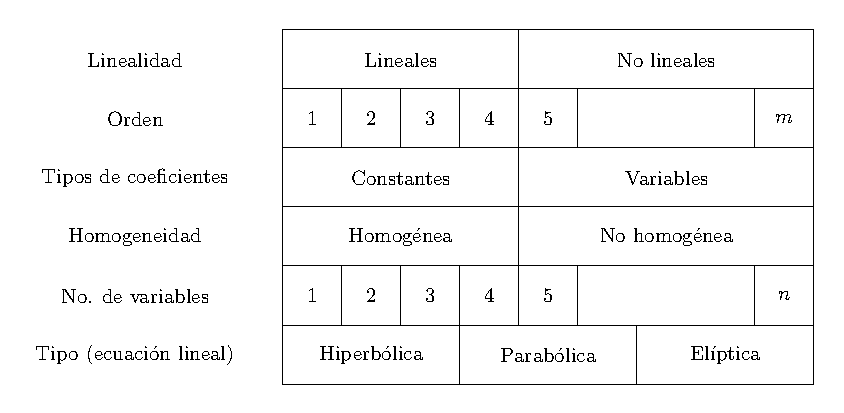
\includegraphics[scale=0.87]{Imagenes/Cuadro_Clasificacion_EDP.eps}
    \caption{Diagrama de clasificación de EDP.}
    \label{fig:figura_clasificacion_EDP}
\end{figure}
\end{frame}
\end{document}